% Modelo de relatório no estilo artigo em duas colunas
\documentclass[twocolumn]{article}
\usepackage[utf8]{inputenc}
\usepackage{amsmath}
\usepackage{subcaption}
\usepackage{mathtools}
\usepackage{graphicx}
\usepackage{color}
\usepackage{authblk}
\usepackage{lmodern}
% \usepackage[colorlinks,citecolor=black,urlcolor=black,bookmarks=false,hypertexnames=true]{hyperref}
\usepackage[margin=0.9in]{geometry}
\usepackage{pdfpages}
\usepackage{fancyhdr}
\usepackage[utf8]{inputenc}

\usepackage[sorting=none,style=numeric]{biblatex}
\addbibresource{refs.bib}
\usepackage[justification=centering]{caption}
\usepackage{makecell}
\usepackage{booktabs}
\usepackage{hhline}
\usepackage{amsmath}
\usepackage{amssymb}
\usepackage{soul}
\usepackage{gensymb}
\usepackage{listings}

\setlength\parindent{0pt}


\newcommand{\myname}{Nishant Aswani}
\newcommand{\mynetid}{nsa325}
\newcommand{\myemail}{nsa325@nyu.edu}
\newcommand{\myhwtype}{Lab }
\newcommand{\myhwnum}{8}
\newcommand{\mycoursenumber}{ENGR-UH 3511}
\newcommand{\myclassname}{Computer Organization and Architecture}
\newcommand{\myassignmenttitle}{Cache Memory and Design Choices}
\newcommand{\myinstructor}{Cristoforos Vasilatos}

\newcommand{\cc}[1]{\texttt{#1}}

\lstset{
  basicstyle=\ttfamily,
  escapeinside=||
}

% Tamanho das margens:
% \geometry{
% 	a4paper,
% 	total={170mm,257mm},
% 	left=30mm,
% 	top=20mm,
% }
%%%%%%%%%%%%%%%%%%%%%%%%%%%%%%%%%%%%%%%%%
% Bibliografia estilo ABNT. Se não tiver instalado, comente a linha abaixo.
% \usepackage[alf, abnt-etal-list=0, abnt-emphasize=bf,abnt-last-names=bibtex, abnt-etal-text=it, abnt-etal-cite=2]{abntex2cite}
%%%%%%%%%%%%%%%%%%%%%%%%%%%%%%%%%%%%%%%%%

% Dados de identificação
\title{\myassignmenttitle}
\author{\myname, \myemail}
\affil{\myclassname (\mycoursenumber), Instructor \myinstructor}
\date{}

\begin{document}
%%%%%%%%%%%%%%%%%%%%%%%%%%%%%%%%%%%%%%%%%%%%%%%% COVER PAGE %%%%%%%%%%%%%%%%%%%%%%%%%%%%%%%%%%%%%%%%%%%%%%%%%%%%
\onecolumn
\pagestyle{fancy}
\fancyhf{}
\renewcommand{\headrulewidth}{0pt}
\rhead{\textbf{Division of Engineering}}
\lhead{\textbf{NYU Abu Dhabi}}

\begin{center}
  
\includegraphics[scale=0.15]{etc/NYUAD-alt-logo.jpg}
\end{center}

{\vspace{2.5em}}

\begin{center}
    \Huge{\textbf{\mycoursenumber}}\\
    {\vspace{0.5em}}
    \Huge{\textbf{\myclassname}}
\end{center}

{\vspace{10em}}

\begin{center}
  \begin{tabular}{|rp{5.0cm}lll|}
    \hline
    &  &  &  & \\
    &  &  &  & \\
    \Large{\textbf{Name:}} & \Large{\myname}
    
    \  &  &  & \\
    \Large{\textbf{Net ID:}} & \Large{\mynetid}
    
    \  &  &  & \\
    \Large{\textbf{Assignment Title:}} & \Large{\myhwtype \myhwnum}
    
    \
    
    \  &  &  & \\
    \hline
  \end{tabular}
\end{center}

\

{\newpage}
%%%%%%%%%%%%%%%%%%%%%%%%%%%%%%%%%%%%%%%%%%%%%%%% COVER PAGE %%%%%%%%%%%%%%%%%%%%%%%%%%%%%%%%%%%%%%%%%%%%%%%%%%%%

\maketitle        

% Resumo de no máximo 200 palavras
% \begin{abstract}
% Este documento orienta a descrição das atividades práticas desenvolvidas em laboratório. São usados como exemplo conceitos da Aula 01 de Acionamentos Elétricos sobre partida direta de motor de indução trifásico. Nesta atividade, um motor é acionado com conexões estrela e triângulo a vazio. As correntes nominais e de partida são medidas com amperímetro analógico e comparadas entre si. Nota-se que, mesmo sem carga, as corrente em estrela são maiores. 
% \end{abstract}

\section{Introduction}

Cache is a microarchitecture concept that allows for quicker access between the processor and memory by exploiting spatio-temporal locality. Chunks of data from memory is stored at points in between the processor and memory allowing for quick access. \\

As with most design options, varying the cache designs results in the differing resulting metrics and trade-offs, such as a lower miss rate or lower miss penalty. This lab explores these metric outputs, defines a cost function, and optimizes cache design to minimize for the designed cost metric. 

\section{Testing Configurations}

If settings for a cache are not specificed, assume default

% \subsection{L1 Unified vs. Separate}

% \textbf{Separate}
% \begin{lstlisting}
% L1 instruction cache:   il1:256:32:1:l    (8 KB)
% L1 data cache:          dl1:256:32:1:l    (8 KB)
% L2 unified cache:       ul2:1024:64:4:l   (256 KB)
% \end{lstlisting}

% \textbf{Unified}
% \begin{lstlisting}
% L1 unified cache:       ul1:256:32:1:l    (8 KB)
% L2 unified cache:       ul2:1024:64:4:l   (256 KB)
% \end{lstlisting}

% The unified implementation was not possible because a bug in the simulator does not allow for a fully unified cache, despit there being examples showing how to do it.

\subsection{Unequal I and D cache sizes}

\textbf{Larger D cache}
\begin{lstlisting}
L1 instruction cache:   il1:128:32:1:l    (4 KiB)
L1 data cache:          dl1:256:32:1:l    (8 KiB)
\end{lstlisting}

\textbf{Larger I cache}
\begin{lstlisting}
L1 instruction cache:   il1:256:32:1:l    (8 KiB)
L1 data cache:          dl1:128:32:1:l    (4 KiB)
\end{lstlisting}

In this case, this would likely impact the performance by increasing the miss rate of the smaller cache.\\

\begingroup
    \medskip
    \centering
    \def\arraystretch{1.5}
        \scriptsize{
        \begin{tabular}{llll}
            \toprule
            IL1 Cache Size & IL1 Miss Rate(\%) & DL1 Cache Size  & DL1 Miss Rate(\%)\\
             \midrule
            4KB & 6.5 & 8KB & 7.2\\
            8KB & 4.9 & 4KB & 10.99\\
            \bottomrule
        \end{tabular}
        }
    \captionof{table}{Miss rate of varying IL1 and DL1 cache size}
    \label{fig:noOptimization}
    \medskip
\endgroup

\newpage

\subsection{Increasing Associativity}

\textbf{Direct-Mapped (1-way)}
\begin{lstlisting}
L2 unified cache:       ul2:4096:64:1:l   (256 KiB)
\end{lstlisting}

\textbf{2-way Associativity}
\begin{lstlisting}
L2 unified cache:       ul2:2048:64:2:l   (256 KiB)
\end{lstlisting}

\textbf{4-way Associativity}
\begin{lstlisting}
L2 unified cache:       ul2:1024:64:4:l   (256 KiB)
\end{lstlisting}

\textbf{8-way Associativity}
\begin{lstlisting}
L2 unified cache:       ul2:512:64:8:l   (256 KiB)
\end{lstlisting}

\textbf{16-way Associativity}
\begin{lstlisting}
L2 unified cache:       ul2:256:64:16:l   (256 KiB)
\end{lstlisting}
\medskip
The results clearly show that there is a diminishing returns in increasing the associativity. Also, we know that increasing associativity raises the cost in terms of hardware because more comparators are needed.\\

\begingroup
    \medskip
    \centering
    \def\arraystretch{1.5}
        \scriptsize{
        \begin{tabular}{ll}
            \toprule
            Set Associativity & UL2 Miss Rate(\%) \\
             \midrule
            1 & 7.15\\
            2 & 4.15\\
            4 & 3.13\\
            8 & 2.87\\
            16 & 2.75\\
            \bottomrule
        \end{tabular}
        }
    \captionof{table}{Miss rate of varying UL2 associativity}
    \label{fig:noOptimization}
    \medskip
\endgroup

\subsection{Comparing Replacement Policies and Increasing UL2 Size}

For the L2 unified caches below, the three replacement policies (LRU, FIFO, and R) were benchmarked:

\begin{lstlisting}
L2 unified cache:       ul2:1024:64:4:l   (256 KiB)
L2 unified cache:       ul2:1024:128:4:l   (512 KiB)
L2 unified cache:       ul2:1024:256:4:l   (1024 KiB == 1 MiB)
\end{lstlisting}
\medskip
The results show that increasing the size of the cache decreases the miss rate and LRU is the better replacement by far the best replacement policy at various cache sizes and its benefits increase as the cache size increases\\

\begingroup
    \medskip
    \centering
    \def\arraystretch{1.5}
        \scriptsize{
        \begin{tabular}{llc}
            \toprule
            UL2 Cache Size & Policy & UL2 Miss Rate(\%) \\
             \midrule
            & LRU & 3.13\\
            256 KB & FIFO & 3.64\\
            & Random & 3.95\\
            \midrule
            & LRU & 1.60\\
            512 KB & FIFO & 1.83\\
            & Random & 1.93\\
            \midrule
            & LRU & 0.59\\
            1024 KB & FIFO & 0.71\\
            & Random & 0.76 \\
            \bottomrule
        \end{tabular}
        }
    \captionof{table}{Miss rate of varying UL2 replacement policy}
    \label{fig:noOptimization}
    \medskip
\endgroup

\section{Calculating CPI}

\bigskip

\textbf{CPI Calculation for GCC}
\begin{lstlisting}
IL1 Miss Rate: 0.47%
DL1 Miss Rate: 1.05%
UL2 Miss Rate: 12.30%
L1 Miss Penalty: 5 cycles
L2 Miss Penalty: 20 cycles
Base CPI: 1 cycle
Load & stores are 36.1% of instructions

L1 instruction cache:   il1:512:64:2:f   (64 KiB)
L1 data cache:          dl1:512:64:2:f    (64 KiB)
L2 unified cache:       ul2:16384:64:1:f   (1 MiB)

IL1 CPI = IL1 Miss Rate * IL1 Miss Penalty = 0.0047 * 5 = 0.0235

DL1 CPI = DL1 Miss Rate * DL1 Miss Penalty * Load/Store % = 0.0105 * 5 * 0.361
= 0.0189525

UL2 CPI = (IL1 Miss Rate + DL1 Miss Rate * Load/Store %) * UL2 Miss Rate * 
UL2 Miss Penalty = (0.0047 + 0.0105 * 0.361) * 0.1230 * 20 = 0.0209

Total CPI = Base CPI + IL1 CPI + DL1 CPI + UL2 CPI
Total CPI = 1 + 0.0235 + 0.0189 + 0.0209 = 1.063
\end{lstlisting}
\bigskip
\bigskip


\textbf{CPI Calculation for GO}
\begin{lstlisting}
IL1 Miss Rate: 0.13%
DL1 Miss Rate: 0.08%
UL2 Miss Rate: 7.22%
L1 Miss Penalty: 5 cycles
L2 Miss Penalty: 20 cycles
Base CPI: 1 cycle
Load & stores are 38.8% of instructions

L1 instruction cache:   il1:512:64:2:f   (64 KiB)
L1 data cache:          dl1:512:64:2:f    (64 KiB)
L2 unified cache:       ul2:16384:64:1:f   (1 MiB(

IL1 CPI = IL1 Miss Rate * IL1 Miss Penalty = 0.0013 * 5 = 0.0065

DL1 CPI = DL1 Miss Rate * DL1 Miss Penalty * Load/Store % = 0.0008 * 5 * 0.388
= 0.0016

UL2 CPI = (IL1 Miss Rate + DL1 Miss Rate * Load/Store %) * UL2 Miss Rate * 
UL2 Miss Penalty = (0.0013 + 0.0008 * 0.388) * 0.0722 * 20 = 0.0023

Total CPI = Base CPI + IL1 CPI + DL1 CPI + UL2 CPI
Total CPI = 1 + 0.0065 + 0.0016 + 0.0023 = 1.010
\end{lstlisting}


\newpage

\section{Designing a Cost Function}

\begin{lstlisting}
    -- 4% increase in cost for using a better policy. They are listed worst to
       best (Random, FIFO, LRU)
    -- 6% increase in cost at each associativity level in the L1 cache
    -- 3% increase in cost at each associativity level in the L2 cache
    -- Cost of unified: 2 units; cost of split: 4 units (under the assumption 
       that the benefit of split is lower latency due to pipelined CPU)
    
\end{lstlisting}

\section{Optimizing Cost/Performance}
\textbf{Assumptions}
\begin{lstlisting}
-- 128KB of L1 separate; 1MB of L2 unified
-- Base CPI = 1 cycle; Cache miss penalty: 10 cycles for L1, 100 cycles for L2
-- Fix the block size parameter to 64 bytes
-- GCC Benchmark

Base Costs (Cheapest Levels)
-- Cost of Associativity of 1 at L1 = 5; at L2 = 5
-- Cost of Random Policy = 5
-- Cost of Unified = 2

17 units is the cheapest cache design with 1.1811 CPI as the worst performance. 
This is used as the baseline to calculate performance.
\end{lstlisting}

\begingroup
    \medskip
    \centering
    \def\arraystretch{1.5}
        \scriptsize{
        \begin{tabular}{cccccccc}
            \toprule
            Policy & L1 Block Size:Assoc & IL2 Block Size:Assoc & DL2 Block Size:Assoc & Unified L2 (Y/N) & CPI & Cost & Cost/Performance\\
            \midrule
            Random & 2048:1 & 16384:1 & N/A & Y & 1.1811 & 17   & 1.0000\\
            Random & 1024:2 & 16384:1 & N/A & Y & 1.1309 & 17.3 & 0.9744\\
            Random & 512:4 & 16384:1 & N/A & Y  & 1.1180 & 17.9 & 0.9967 \\
            Random & 256:8 & 16384:1 & N/A & Y  & 1.1113 & 19.1 & 1.0571\\
            \midrule
            Random & 2048:1 & 4096:4 & N/A & Y & 1.1287 & 17.45 & 0.9809\\
            Random & 1024:2 & 4096:4 & N/A & Y & 1.0984& 17.75  & \textbf{0.9710}\\
            Random & 512:4 & 4096:4 & N/A & Y & 1.0872& 18.35   & 0.9936\\
            Random & 256:8 & 4096:4 & N/A & Y & 1.0852& 19.55   & 1.0566\\
            \midrule
            FIFO & 2048:1 & 16384:1 & N/A & Y & 1.1811 & 17.2 & 1.0117\\
            FIFO & 1024:2 & 16384:1 & N/A & Y & 1.1324 & 17.5 & 0.9870\\
            FIFO & 512:4 & 16384:1 & N/A & Y & 1.1192 & 18.1 & 1.0089\\
            FIFO & 256:8 & 16384:1 & N/A & Y & 1.1132 & 19.3 & 1.0700\\
            \midrule
            FIFO & 2048:1 & 4096:4 & N/A & Y & 1.1256 & 17.65 & 0.9894\\
            FIFO & 1024:2 & 4096:4 & N/A & Y & 1.0937 & 17.95 & 0.9777\\
            FIFO & 512:4 & 4096:4 & N/A & Y & 1.0843 & 18.55  & 1.0017\\
            FIFO & 256:8 & 4096:4 & N/A & Y & 1.0804 & 19.75  & 1.0627\\
            \midrule
            LRU & 2048:1 & 16384:1 & N/A & Y & 1.1811 & 17.4 & 1.0235\\
            LRU & 1024:2 & 16384:1 & N/A & Y & 1.1252& 17.7 & 0.9919\\
            LRU & 512:4 & 16384:1 & N/A &  Y & 1.1073& 18.3   & 1.0092\\
            LRU & 256:8 & 16384:1 & N/A &  Y & 1.0995 & 19.5 & 1.0678\\
            \midrule
            LRU & 2048:1 & 4096:4 & N/A & Y & 1.1186& 17.85 & 0.9944\\
            LRU & 1024:2 & 4096:4 & N/A & Y & 1.0851& 18.15 & 0.9809\\
            LRU & 512:4 & 4096:4 & N/A &  Y & 1.0735& 18.75 & 1.0024\\
            LRU & 256:8 & 4096:4 & N/A &  Y & 1.0693& 19.95 & 1.0624\\
             
            \bottomrule
        \end{tabular}
        }
    \captionof{table}{General search for favorable parameters}
    \label{table:generalResults}
    \medskip
\endgroup

Looking at the table \ref{table:generalResults}, we can hone in and use parameters that favor 2 way associativity for L1 and explore more options for associativity at L2. We will keep the unified structure L2 structure and continue to test for all three policies.

\begingroup
    \medskip
    \centering
    \def\arraystretch{1.5}
        \scriptsize{
        \begin{tabular}{cccccccc}
            \toprule
            Policy & L1 Block Size:Assoc & IL2 Block Size:Assoc & DL2 Block Size:Assoc & Unified L2 (Y/N) & CPI & Cost & Cost/Performance\\
            \midrule
            Random & 1024:2 & 16384:1 & N/A & Y & 1.1309 & 17.3 & 0.9744\\
            Random & 1024:2 & 8192:2 & N/A & Y & 1.1051 & 17.45 & \textbf{0.9604}\\
            Random & 1024:2 & 4096:4 & N/A & Y & 1.0984 & 17.75  & 0.9710\\
            Random & 1024:2 & 2048:8 & N/A & Y & 1.0943 & 18.35 & 1.0000\\
            \midrule
            FIFO & 1024:2 & 16384:1 & N/A & Y & 1.1324 & 17.5 & 0.9870\\
            FIFO & 1024:2 & 8192:2 & N/A & Y & 1.1020 & 17.65 & 0.9687\\
            FIFO & 1024:2 & 4096:4 & N/A & Y & 1.0937 & 17.95 & 0.9777\\
            FIFO & 1024:2 & 2048:8 & N/A & Y & 1.0877 & 18.55 & 1.0049\\
            \midrule
            LRU & 1024:2 & 16384:1 & N/A & Y & 1.1811 & 17.4 & 0.9919\\
            LRU & 1024:2 & 8192:2 & N/A & Y & 1.0953 & 17.85 & 0.9737\\
            LRU & 1024:2 & 4096:4 & N/A & Y & 1.0851& 18.15 & 0.9809\\
            LRU & 1024:2 & 2048:8 & N/A & Y & 1.0777 & 18.75 & 1.0064\\
            \bottomrule
        \end{tabular}
        }
    \captionof{table}{Targeted search for favorable parameters}
    \label{table:targetedResults}
    \medskip
\endgroup

\section{Discussion \& Conclusion}

Looking at the results of table \ref{table:targetedResults}, we see that a unified L2 cache, with a 2 way associativity at L1 and L2, following a random policy has the best cache configuration for this cost function. Testing for the separate cache was not done because it was inferred that the increase in cost would outweigh any minor CPI improvement.\\ 

It is most likely that the cost function designed here was too costly for increasing policy. Despite LRU performing quite well in decreasing the CPI, its benefit was ultimately lost due to the high cost. More obviously, the cost function was also biased towards a unified L2 cache. Updating the cost function to reduce these biases would most likely support a cache configuration using FIFO. In the case of the GCC benchmark, a separate cache may have also been beneficial as the instruction/data split is unequal. Hence, separately configurable L2 caches may have provided a slight benefit.  

% \begingroup
%     \centering
%     \medskip
%     %width=\columnwidth
%     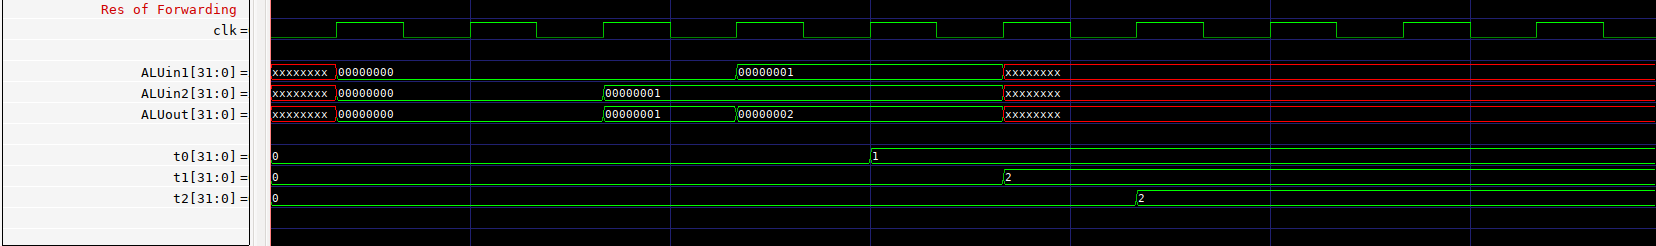
\includegraphics[width=\columnwidth]{Lab-Tex/Lab7-images/p2.png}
%     \captionof{figure}{Resulting values of forwarding}
%     \label{fig:forwarding_res}
%     \medskip
% \endgroup


%%%%%%%%%%%%%%%%%%%%%%%%%%5
% BIBLIOGRAFIA 
% Estilo de bibliografia ABNT. Se não tiver instalado, mude para plain ou ieeetr

%\bibliographystyle{plain} % Inclua isso se não tiver ABNTEX instalado
% \begin{thebibliography}{refs}
% \bibitem{}
\printbibliography
% \end{thebibliography}
\end{document}